\section{Why is Speculative Planning Expensive?}

\textbf{Speculative planning} extends the principle of speculative execution to multi-step sequential decision making in LLM-based agents. This approach employs a dual-agent architecture with a ``draft-and-verify'' paradigm to accelerate planning while preserving solution quality. In this framework, a computationally efficient $\approxi$ rapidly generates a sequence of candidate actions $k$, while simultaneously the more capable $\target$ (the original planning agent) utilizes the prefix trajectory from the $\approxi$ to simultaneously generate its own next actions as verification of the proposals of $\approxi$'. 
%$\target$ utilizes the prefix trajectory from the $\approxi$ while simultaneously generating its own next actions. 
This parallel processing architecture enables multiple verification steps to proceed concurrently rather than sequentially. 
% The system continuously compares the action trajectories from both agents. 
When $\target$ confirms alignment with $\approxi$'s proposals, those actions are immediately committed to the final plan. This verification process proceeds in parallel threads, significantly reducing the end-to-end latency compared to traditional autoregressive planning. Whenever divergence occurs, where $\target$ proposes a different action than the $\approxi$, the system adopts $\target$'s alternative and continues planning from this corrected trajectory. This mechanism ensures that the final execution path always conforms to $\target$'s policy 
%while leveraging $\approxi$'s predictions to reduce waiting time. 
%By parallelizing verification, speculative planning 
while achieve substantial acceleration. 
%without compromising solution integrity.

%utilizes the idea of speculative execution on agent planning step level. It leverages the ``draft-and-verify'' strategy to the domain of multi-step sequential decision making. A lightweight approximation agent begins drafting up to $k$ candidate actions in a row, and the stronger target agent which is originally the agent utilizes prefix steps generated by the approximation agent and generate the next step at the same time. This is done for verification which is done by by comparing whether actions proposed by approximation and target agents match with each other. Each step of target agent utilize the prefix trajectory generated by the approximation agent, thus these target agent's steps are run in parallel threads. As tokens stream in, the system continuously compares the two trajectories. Any longest prefix that the target agent confirms is committed instantly, and both agents continue from that new verified trajectory; if the target diverges at some step, its alternative replaces the draft, ensuring that final execution matches the target agent's policy. 
%By interleaving generation and verification in this way, speculative planning transforms a strictly serial planning loop into an effectively parallel procedure, delivering substantial wall-clock speed-ups without degrading solution quality.

\begin{figure}
    \centering
    \begin{subfigure}[b]{0.48\textwidth}
        \centering
        \resizebox{\linewidth}{!}{\small
\begin{tikzpicture}
    \node (step1) at (-5,-1.5) [rectangle, draw=lightblue!50, fill=lightblue!50, minimum width=25pt, minimum height=12pt, inner sep=0pt, anchor=west] {};
    \node (exc1) at (step1.east) [rectangle, draw=black!30, fill=black!30, minimum width=5pt, minimum height=12pt, inner sep=0pt, anchor=west] {};
    \node (step2) at (exc1.east) [rectangle, draw=lightblue!50, fill=lightblue!50, minimum width=20pt, minimum height=12pt, inner sep=0pt, anchor=west] {};
    \node (exc2) at (step2.east) [rectangle, draw=black!30, fill=black!30, minimum width=5pt, minimum height=12pt, inner sep=0pt, anchor=west] {};
    
    
    \node at (-6.3,-1.5) {\textcolor{blue!80!black}{Approximation}};

    \node (plan1) at (step1.east) [yshift=15pt] {\textcolor{blue!80!black}{\scriptsize \makecell{Plan A\\$\downarrow$}}};
    \node (plan2) at (step2.east) [yshift=15pt] {\textcolor{blue!80!black}{\scriptsize \makecell{Plan B\\$\downarrow$}}};
    
    % \node (plan5) at (step5.east) [yshift=15pt] {\textcolor{blue!80!black}{\scriptsize \makecell{Plan E\\$\downarrow$}}};

    

    \node (tar_step1) at ([yshift=-40pt]step1.west) [rectangle, draw=lightorange!50, fill=lightorange!50, minimum width=58pt, minimum height=12pt, inner sep=0pt, anchor=west] {};
    \node (tar_step2) at ([yshift=-55pt]step2.west) [rectangle, draw=lightorange!50, fill=lightorange!50, minimum width=55pt, minimum height=12pt, inner sep=0pt, anchor=west] {};
    
    % \node (tar_step5) at ([yshift=-100pt]step5.west) [rectangle, draw=lightorange!50, fill=lightorange!50, minimum width=25pt, minimum height=12pt, inner sep=0pt, anchor=west] {};
    
    \node at (-6.3,-3) {\textcolor{orange!80!black}{Target}};


    \node (step3) at (tar_step2.east|- step1) [rectangle, draw=lightblue!50, fill=lightblue!50, minimum width=30pt, minimum height=12pt, inner sep=0pt, anchor=west] {};
    \node (exc3) at (step3.east) [rectangle, draw=black!30, fill=black!30, minimum width=5pt, minimum height=12pt, inner sep=0pt, anchor=west] {};
    \node (step4) at (exc3.east) [rectangle, draw=lightblue!50, fill=lightblue!50, minimum width=23pt, minimum height=12pt, inner sep=0pt, anchor=west] {};
    \node (exc4) at (step4.east) [rectangle, draw=black!30, fill=black!30, minimum width=5pt, minimum height=12pt, inner sep=0pt, anchor=west] {};
    % \node (step5) at (exc4.east) [rectangle, draw=lightblue!50, fill=lightblue!50, minimum width=19pt, minimum height=12pt, inner sep=0pt, anchor=west] {};
    % \node (exc5) at (step5.east) [rectangle, draw=black!30, fill=black!30, minimum width=5pt, minimum height=12pt, inner sep=0pt, anchor=west] {};
    \node (plan3) at (step3.east) [yshift=15pt] {\textcolor{blue!80!black}{\scriptsize \makecell{Plan C\\$\downarrow$}}};
    \node (plan4) at (step4.east) [yshift=15pt] {\textcolor{blue!80!black}{\scriptsize \makecell{Plan D\\$\downarrow$}}};
    \node (tar_step3) at ([yshift=-40pt]step3.west) [rectangle, draw=lightorange!50, fill=lightorange!50, minimum width=70pt, minimum height=12pt, inner sep=0pt, anchor=west] {};
    \node (tar_step4) at ([yshift=-55pt]step4.west) [rectangle, draw=lightorange!50, fill=lightorange!50, minimum width=80pt, minimum height=12pt, inner sep=0pt, anchor=west] {};
    \node (tar_exc4) at (tar_step4.east) [rectangle, draw=black!30, fill=black!30, minimum width=5pt, minimum height=12pt, inner sep=0pt, anchor=west] {};

    \draw [->, thick] (-7,-4) -- node [below, xshift=140pt, yshift=-3pt] {Time} (3,-4);
    \draw [-, dashed, thick] ([yshift=10pt]step1.west) -- node [yshift=-48pt] {\scriptsize step 1} ++(0,-2.8);
    \draw [-, dashed, thick] ([yshift=10pt]step2.west) -- node [yshift=-48pt] {\scriptsize step 2} ++(0,-2.8);
    \draw [-, dashed, thick] ([yshift=10pt]step3.west) -- node [yshift=-48pt] {\scriptsize step 3} ++(0,-2.8);
    \draw [-, dashed, thick] ([yshift=10pt]step4.west) -- node [yshift=-48pt] {\scriptsize step 4} ++(0,-2.8);
    
    % \draw [-, dashed, thick] ([yshift=10pt]step5.west) -- node [yshift=-68pt] {\scriptsize step 5} ++(0,-4.4);
    % \draw [-, solid, thick, draw=red, line width=1.5pt] ([yshift=6pt]tar_step3.east) -- node [yshift=-36pt] {\scriptsize \textcolor{red}{\makecell{Cancel\\plan}}} ++(0,-1.75);

    \node (tar_plan1) at (tar_step1.east) [yshift=15pt] {\textcolor{orange!80!black}{\scriptsize \makecell{Plan A \textcolor{green!80!black}{\checkmark}\\$\downarrow$}}};
    \node (tar_plan2) at (tar_step2.east) [yshift=15pt] {\textcolor{orange!80!black}{\scriptsize \makecell{Plan B \textcolor{green!80!black}{\checkmark}\\$\downarrow$}}};
    \node (tar_plan3) at (tar_step3.east) [yshift=15pt] {\textcolor{orange!80!black}{\scriptsize \makecell{Plan C \textcolor{green!80!black}{\checkmark}\\$\downarrow$}}};
    \node (tar_plan4) at (tar_step4.east) [yshift=15pt] {\textcolor{red}{\scriptsize \makecell{Plan D \ding{55}\\$\downarrow$}}};
    \draw [<->, thick]([yshift=0pt]step1.west |- 0,-4.8) -- node [below] {Long total task time}   ([yshift=0pt]tar_exc4.east |- 0,-4.8);
    
\end{tikzpicture}
}
        \captionsetup{skip=2pt}
        \caption{speculative step too small ($k = 2$).}
    \end{subfigure}
    \hfill
    \begin{subfigure}[b]{0.46\textwidth}
        \centering
        \resizebox{\linewidth}{!}{\small
\begin{tikzpicture}
    \node (step1) at (-5,0) [rectangle, draw=lightblue!50, fill=lightblue!50, minimum width=25pt, minimum height=12pt, inner sep=0pt, anchor=west] {};
    \node (exc1) at (step1.east) [rectangle, draw=black!30, fill=black!30, minimum width=5pt, minimum height=12pt, inner sep=0pt, anchor=west] {};
    \node (step2) at (exc1.east) [rectangle, draw=lightblue!50, fill=lightblue!50, minimum width=20pt, minimum height=12pt, inner sep=0pt, anchor=west] {};
    \node (exc2) at (step2.east) [rectangle, draw=black!30, fill=black!30, minimum width=5pt, minimum height=12pt, inner sep=0pt, anchor=west] {};
    \node (step3) at (exc2.east) [rectangle, draw=lightblue!50, fill=lightblue!50, minimum width=30pt, minimum height=12pt, inner sep=0pt, anchor=west] {};
    \node (exc3) at (step3.east) [rectangle, draw=black!30, fill=black!30, minimum width=5pt, minimum height=12pt, inner sep=0pt, anchor=west] {};
    \node (step4) at (exc3.east) [rectangle, draw=lightblue!50, fill=lightblue!50, minimum width=23pt, minimum height=12pt, inner sep=0pt, anchor=west] {};
    \node (exc4) at (step4.east) [rectangle, draw=black!30, fill=black!30, minimum width=5pt, minimum height=12pt, inner sep=0pt, anchor=west] {};
    \node (step5) at (exc4.east) [rectangle, draw=lightblue!50, pattern=north west lines, pattern color=lightblue!100, minimum width=19pt, minimum height=12pt, inner sep=0pt, anchor=west] {};
    \node (exc5) at (step5.east) [rectangle, draw=black!30, pattern=north west lines, pattern color=black!100, minimum width=5pt, minimum height=12pt, inner sep=0pt, anchor=west] {};
    \node at (-6.3,0) {\textcolor{blue!80!black}{Approximation}};
    \node (step6) at (exc5.east) [rectangle, draw=lightblue!50, pattern=north west lines, pattern color=lightblue!100, minimum width=19pt, minimum height=12pt, inner sep=0pt, anchor=west] {};
    \node (exc6) at (step6.east) [rectangle, draw=black!30, pattern=north west lines, pattern color=black!100, minimum width=5pt, minimum height=12pt, inner sep=0pt, anchor=west] {};
    \node at (-6.3,0) {\textcolor{blue!80!black}{Approximation}};

    \node (plan1) at (step1.east) [yshift=15pt] {\textcolor{blue!80!black}{\scriptsize \makecell{Plan A\\$\downarrow$}}};
    \node (plan2) at (step2.east) [yshift=15pt] {\textcolor{blue!80!black}{\scriptsize \makecell{Plan B\\$\downarrow$}}};
    \node (plan3) at (step3.east) [yshift=15pt] {\textcolor{blue!80!black}{\scriptsize \makecell{Plan C\\$\downarrow$}}};
    \node (plan4) at (step4.east) [yshift=15pt] {\textcolor{blue!80!black}{\scriptsize \makecell{Plan D\\$\downarrow$}}};
    \node (plan5) at (step5.east) [yshift=15pt] {\textcolor{blue!80!black}{\scriptsize \makecell{Plan E\\$\downarrow$}}};
    \node (plan6) at (step6.east) [yshift=15pt] {\textcolor{blue!80!black}{\scriptsize \makecell{Plan F\\$\downarrow$}}};

    \node (tar_step1) at ([yshift=-40pt]step1.west) [rectangle, draw=lightorange!50, fill=lightorange!50, minimum width=58pt, minimum height=12pt, inner sep=0pt, anchor=west] {};
    \node (tar_step2) at ([yshift=-55pt]step2.west) [rectangle, draw=lightorange!50, fill=lightorange!50, minimum width=55pt, minimum height=12pt, inner sep=0pt, anchor=west] {};
    \node (tar_step3) at ([yshift=-70pt]step3.west) [rectangle, draw=lightorange!50, fill=lightorange!50, minimum width=70pt, minimum height=12pt, inner sep=0pt, anchor=west] {};
    \node (tar_step4) at ([yshift=-85pt]step4.west) [rectangle, draw=lightorange!50, fill=lightorange!50, minimum width=80pt, minimum height=12pt, inner sep=0pt, anchor=west] {};
    \node (tar_step5) at ([yshift=-100pt]step5.west) [rectangle, draw=lightorange!50, pattern=north west lines, pattern color=lightorange!100, minimum width=51pt, minimum height=12pt, inner sep=0pt, anchor=west] {};
    \node (tar_step6) at ([yshift=-115pt]step6.west) [rectangle, draw=lightorange!50, pattern=north west lines, pattern color=lightorange!100, minimum width=27pt, minimum height=12pt, inner sep=0pt, anchor=west] {};
    \node (tar_exc4) at (tar_step4.east) [rectangle, draw=black!30, fill=black!30, minimum width=5pt, minimum height=12pt, inner sep=0pt, anchor=west] {};
    \node at (-6.3,-2.8) {\textcolor{orange!80!black}{Target}};

    \draw [->, thick] (-7,-4.5) -- node [below, xshift=140pt, yshift=-3pt] {Time} (3,-4.5);
    \draw [-, dashed, thick] ([yshift=10pt]step1.west) -- node [yshift=-76pt] {\scriptsize step 1} ++(0,-4.8);
    \draw [-, dashed, thick] ([yshift=10pt]step2.west) -- node [yshift=-76pt] {\scriptsize step 2} ++(0,-4.8);
    \draw [-, dashed, thick] ([yshift=10pt]step3.west) -- node [yshift=-76pt] {\scriptsize step 3} ++(0,-4.8);
    \draw [-, dashed, thick] ([yshift=10pt]step4.west) -- node [yshift=-76pt] {\scriptsize step 4} ++(0,-4.8);
    \draw [-, dashed, thick] ([yshift=10pt]step5.west) -- node [yshift=-76pt] {\scriptsize step 5} ++(0,-4.8);
    \draw [-, dashed, thick] ([yshift=10pt]step6.west) -- node [yshift=-76pt] {\scriptsize step 6} ++(0,-4.8);
    \draw [-, solid, thick, draw=red, line width=1.5pt] ([yshift=6pt]tar_step4.east) -- node [yshift=-36pt] {\scriptsize \textcolor{red}{\makecell{Cancel\\plan}}} ++(0,-1.7);

    \node (tar_plan1) at (tar_step1.east) [yshift=15pt] {\textcolor{orange!80!black}{\scriptsize \makecell{Plan A \textcolor{green!80!black}{\checkmark}\\$\downarrow$}}};
    \node (tar_plan2) at (tar_step2.east) [yshift=15pt] {\textcolor{orange!80!black}{\scriptsize \makecell{Plan B \textcolor{green!80!black}{\checkmark}\\$\downarrow$}}};
    \node (tar_plan3) at (tar_step3.east) [yshift=15pt] {\textcolor{orange!80!black}{\scriptsize \makecell{Plan C \textcolor{green!80!black}{\checkmark}\\$\downarrow$}}};
    \node (tar_plan4) at (tar_step4.east) [yshift=15pt] {\textcolor{red}{\scriptsize \makecell{Plan D \ding{55}\\$\downarrow$}}};
    \draw [<->, thick]([yshift=0pt]step1.west |- 0,-5.2) -- node [below] {Short total task time}   ([yshift=0pt]tar_exc4.east |- 0,-5.2);

    \node[minimum height=2pt] at (-6.3,-5.6) {};
\end{tikzpicture}
}
        \captionsetup{skip=2pt}
        \caption{speculative step too large ($k = 6$).}
    \end{subfigure}
    \captionsetup{skip=2pt}
    \caption{Limitations of fix speculative step approaches. A small $k$ limits acceleration although it avoids waste, while a large $k$ increases speedup at the cost of redundant computation when mismatches occur (step 5 \& 6 is wasted in (b)).}
    \label{fig:motivation_k}
    \vspace{-5pt}
\end{figure}

\noindent \textbf{Speculative Planning Cost Broken-Down} ~
While speculative execution offers the promise of improving latency by parallelizing candidate task executions in a lossless manner, it inevitably introduces additional token consumption. As shown in \cref{fig:motivation_k} (b), this overhead becomes particularly significant when $k$ is large, motivating the need for a more adaptive planning approach. In this section, we aim to understand where the major overheads arise by systematically breaking down the costs of speculative planning under different fixed-$k$ settings. 
Redundant costs in speculative planning arise when token consumption does not contribute to the final generated plan or acceleration, which can be divided into four main components: redundant (1) the prompt tokens and (2) the generation tokens consumed by $\approxi$, and (3) the prompt tokens and (4) the generation tokens consumed by $\target$. Figure \ref{fig:cost_composition} provides a detailed breakdown of token consumption for each component, comparing normal planning against fixed-$k$ speculative planning across different $k$s with 2 speculative planning configurations.


% \begin{table}[t]
% \centering
% \caption{Token Cost Comparison Between Planning Methods}
% \label{tab:token-cost}

% \begin{subtable}[t]{\textwidth}
% \centering
% \small
% \caption{Standard Planning}
% \label{tab:standard}
% \begin{tabular}{lrrrrrrr}
% \toprule
% Plan Type & Approx P & Approx G & Target P & Target G & Total P & Total G & Total \\
% \midrule
% Normal & 5979.7 & 107.6 & 12581.5 & 1881.3 & 18561.2 & 1988.9 & 20550.1 \\
% Spec (k=2) & 10759.8 & 165.7 & 18162.7 & 2431.2 & 28922.5 & 2596.9 & 31519.4 \\
% Spec (k=4) & 19894.5 & 281.9 & 26610.1 & 2963.1 & 46504.6 & 3245.1 & 49749.7 \\
% Spec (k=6) & 31113.1 & 349.0 & 32982.6 & 3514.2 & 64095.7 & 3863.3 & 67959.0 \\
% \midrule
% Redund (k=2) & +4780.1 & +58.1 & +5581.2 & +549.9 & +10361.3 & +608.0 & +10969.3 \\
% Redund (k=4) & +13914.8 & +174.3 & +14028.6 & +1081.9 & +27943.4 & +1256.2 & +29199.6 \\
% Redund (k=6) & +25133.3 & +241.5 & +20401.1 & +1633.0 & +45534.5 & +1874.4 & +47408.9 \\
% \bottomrule
% \end{tabular}
% \end{subtable}

% \vspace{10pt}

% \begin{subtable}[t]{\textwidth}
% \centering
% \small
% \caption{OpenAGI (CoT + MultiAgent)}
% \label{tab:openagi}
% \begin{tabular}{lrrrrrrr}
% \toprule
% Plan Type & Approx P & Approx G & Target P & Target G & Total P & Total G & Total \\
% \midrule
% Normal & 5422.5 & 1701.3 & 35968.4 & 7332.8 & 41390.9 & 9034.0 & 50424.9 \\
% Spec (k=2) & 8158.9 & 2435.4 & 50373.5 & 9881.1 & 58532.4 & 12316.5 & 70848.9 \\
% Spec (k=4) & 13799.2 & 3884.8 & 70283.3 & 13253.9 & 84082.5 & 17138.7 & 101221.2 \\
% Spec (k=6) & 26065.3 & 5466.1 & 97668.0 & 18152.8 & 123733.3 & 23618.9 & 147352.2 \\
% \midrule
% Redund (k=2) & +2736.4 & +734.1 & +14405.1 & +2548.3 & +17141.5 & +3282.4 & +20424.0 \\
% Redund (k=4) & +8376.7 & +2183.5 & +34314.9 & +5921.2 & +42691.6 & +8104.7 & +50796.3 \\
% Redund (k=6) & +20642.8 & +3764.9 & +61699.6 & +10820.0 & +82342.4 & +14584.9 & +96927.3 \\
% \bottomrule
% \end{tabular}
% \end{subtable}

% \begin{minipage}{\textwidth}
% \footnotesize
% \textbf{Note:} P=Prompt Tokens, G=Generation Tokens, Redund=Redundant Cost.
% \end{minipage}
% \end{table}

% openagi_react_cost_comp.png

% \begin{table}[t]
% \caption{Big table \qingfeng{Add captions}}
% \label{tab:token-cost}
% \centering
% \subcaptionbox{table 1\label{tab:1}}{
% \resizebox{\textwidth}{!}{
% \begin{tabular}{lrrrrrrr}
% \toprule
% Plan Type & Approx Prompt & Approx Generation & Target Prompt & Target Generation & Total Prompt & Total Generation & Total Token \\
% \midrule
% Normal Plan & 5979.7 & 107.6 & 12581.5 & 1881.3 & 18561.2 & 1988.9 & 20550.1 \\
% SpecPlan (k=2) & 10759.8 & 165.7 & 18162.7 & 2431.2 & 28922.5 & 2596.9 & 31519.4 \\
% SpecPlan (k=4) & 19894.5 & 281.9 & 26610.1 & 2963.1 & 46504.6 & 3245.1 & 49749.7 \\
% SpecPlan (k=6) & 31113.1 & 349.0 & 32982.6 & 3514.2 & 64095.7 & 3863.3 & 67959.0 \\
% \midrule
% Redundant cost (k = 2) & +4780.1 & +58.1 & +5581.2 & +549.9 & +10361.3 & +608.0 & +10969.3 \\
% Redundant cost (k = 4) & +13914.8 & +174.3 & +14028.6 & +1081.9 & +27943.4 & +1256.2 & +29199.6 \\
% Redundant cost (k = 6) & +25133.3 & +241.5 & +20401.1 & +1633.0 & +45534.5 & +1874.4 & +47408.9 \\
% \bottomrule
% \end{tabular}
% }
% }
% \subcaptionbox{table 2\label{tab:2}}{
% \resizebox{\textwidth}{!}{
% \begin{tabular}{lrrrrrrr}
% \toprule
% Plan Type & Approx Prompt & Approx Generation & Target Prompt & Target Generation & Total Prompt & Total Generation & Total Token \\
% \midrule
% Normal Plan & 5422.5 & 1701.3 & 35968.4 & 7332.8 & 41390.9 & 9034.0 & 50424.9 \\
% SpecPlan (k=2) & 8158.9 & 2435.4 & 50373.5 & 9881.1 & 58532.4 & 12316.5 & 70848.9 \\
% SpecPlan (k=4) & 13799.2 & 3884.8 & 70283.3 & 13253.9 & 84082.5 & 17138.7 & 101221.2 \\
% SpecPlan (k=6) & 26065.3 & 5466.1 & 97668.0 & 18152.8 & 123733.3 & 23618.9 & 147352.2 \\
% \midrule
% Redundant cost (k = 2) & +2736.4 & +734.1 & +14405.1 & +2548.3 & +17141.5 & +3282.4 & +20424.0 \\
% Redundant cost (k = 4) & +8376.7 & +2183.5 & +34314.9 & +5921.2 & +42691.6 & +8104.7 & +50796.3 \\
% Redundant cost (k = 6) & +20642.8 & +3764.9 & +61699.6 & +10820.0 & +82342.4 & +14584.9 & +96927.3 \\
% \bottomrule
% \end{tabular}
% }
% }
% \end{table}


%\cref{tab:token-cost} summarizes these costs and their breakdown under different $k$ values. These costs occur through distinct computation profiles for both the approximation and target agents.

\textit{Approximation agent} incurs excessive wasted token generation when the speculative step $k$ exceeds the number of correct steps the agent can generate sequentially. When a mismatch occurs before reaching $k$, all steps that have already been generated based on the invalidated step become wasted. 
% These steps must then be regenerated from the last correct speculation point. 
This effect intensifies under large-$k$ configurations, where the system frequently issues more speculative steps, only to discard them upon early divergence. In experiments where we adopt LLM with direct generation as $\approxi$ and LLM with chain-of-thought (CoT)~\cite{wei2022chain} as $\target$, $\approxi$'s waste primarily stems from prompt tokens rather than generation tokens. This occurs because both agents employ relatively simple planning strategies with moderate generation length while contain lengthy prompts including environment introduction, task descriptions, and past action trajectories.
%the generated tokens are typically more concise, focusing mainly on producing the next selected action. 
Consequently, speculative executions of $\approxi$ incur significantly higher prompt costs than generation costs. 
\begin{figure}
\centering
\begin{subfigure}[b]{0.44\textwidth}
        \centering
        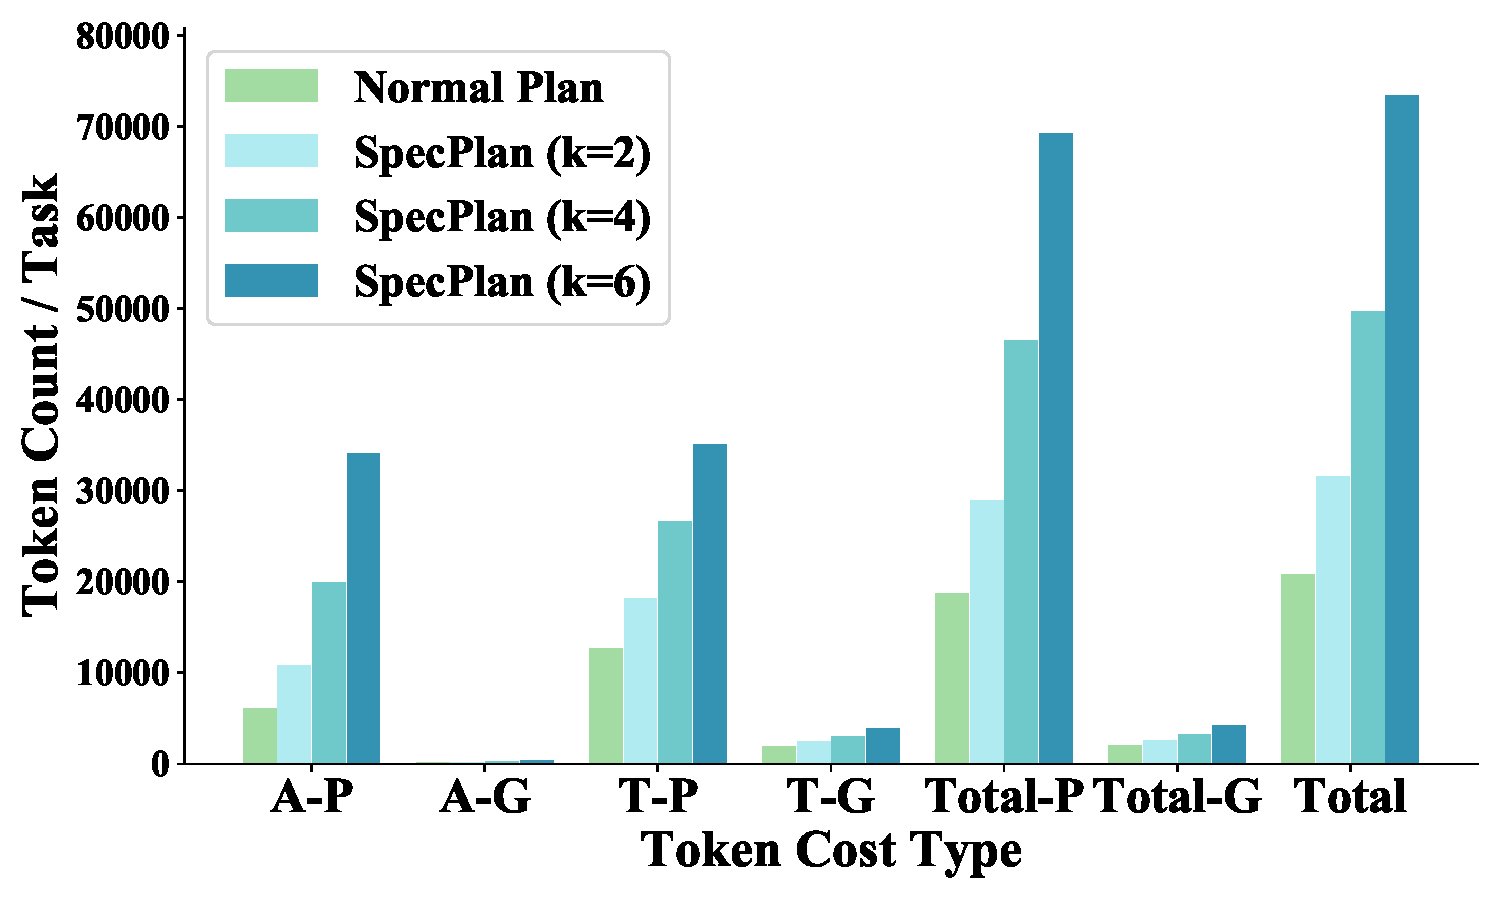
\includegraphics[width=\linewidth]{fig/openagi_react_cost_comp.pdf}
        \captionsetup{skip=1pt}
        \caption{Direct-ReAct}
    \end{subfigure}
    \hfil
    \begin{subfigure}[b]{0.44\textwidth}
        \centering
       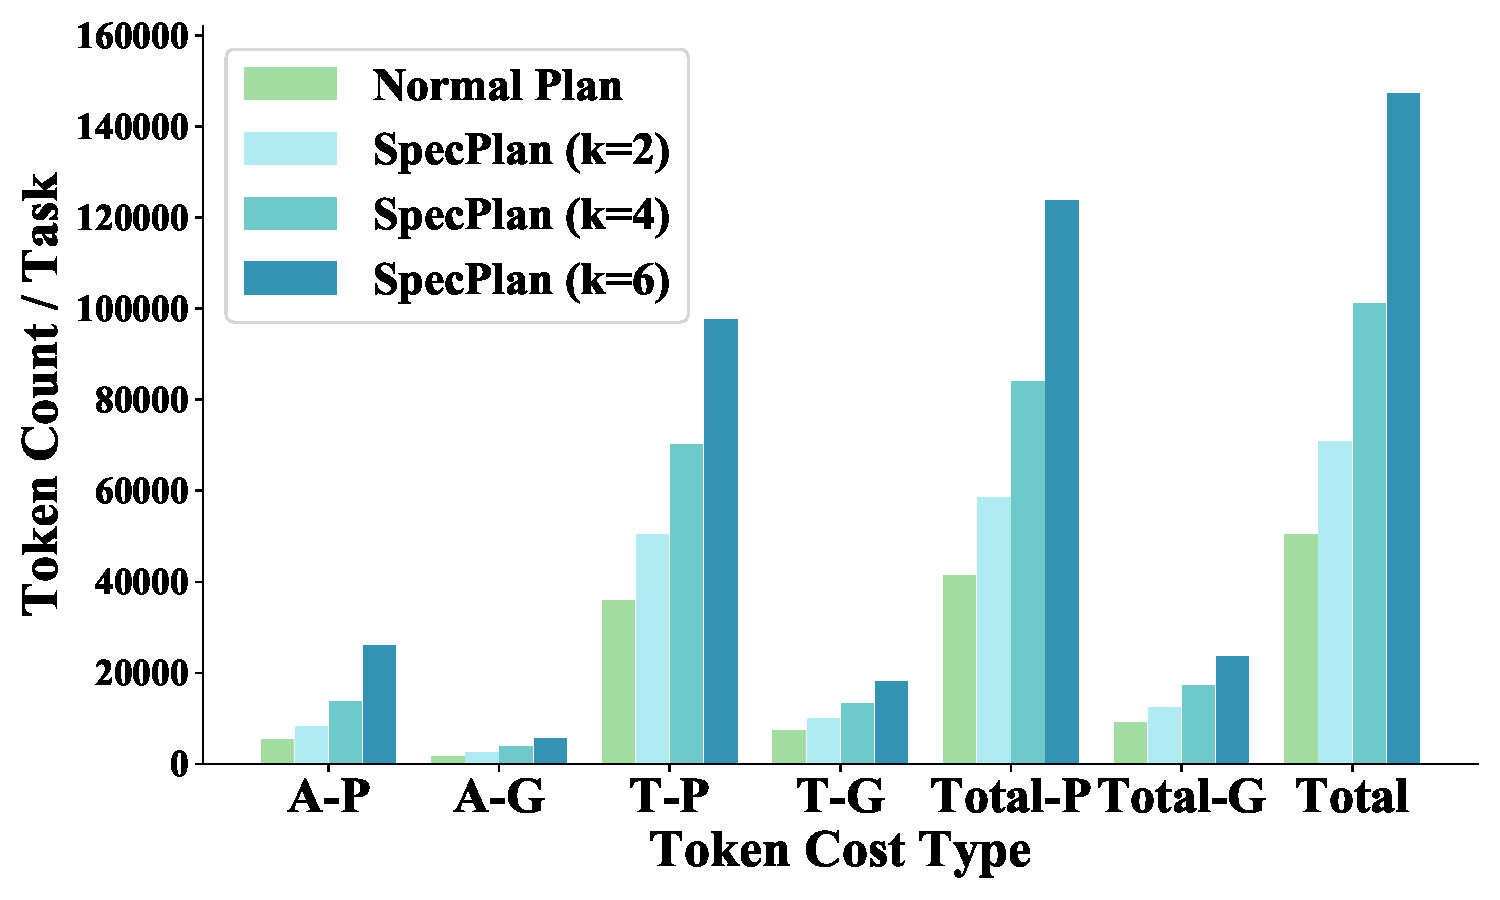
\includegraphics[width=\linewidth]{fig/openagi_mad_cost_comp.pdf}
        \captionsetup{skip=1pt}
        \caption{CoT-MAD}
    \end{subfigure}
\captionsetup{skip=-1pt}
\caption{Token cost breakdown under speculative planning for different fixed $k$ values on the OpenAGI benchmark, shown for two distinct $\approxi$--$\target$ configurations: (a) Direct ($\approxi$) with ReAct ($\target$), and (b) CoT ($\approxi$) with Multi-Agent Debate ($\target$). Each bar contains four segments: $\approxi$’s prompt (A-P) and generation (A-G) tokens, and $\target$’s prompt (T-P) and generation (T-G) tokens. These components are also aggregated into total prompt  (Total-P)and generation tokens (Total-G), and overall total tokens (Total). In both subfigures, higher values of $k$ result in substantially greater total token costs.}
\label{fig:cost_composition}
\end{figure}

\textit{Target agent} also incurs excessive wasted token generation from mismatches between proposed actions from $\approxi$ and $\target$. These mismatches introduce two additional sources of redundant costs: (1) \textbf{Completed $\target$ steps}: When a mismatch occurs at a particular step, all subsequent completed target steps become invalid, rendering their  prompt and generation tokens entirely wasted. (2) \textbf{Ongoing target steps}: All subsequent in-progress target steps after a mismatch are immediately canceled. These steps may have already initiated LLM calls, consumed prompt tokens, and generated partial outputs before forced cancellation. This type of waste grows proportionally with $k$ because Speculative Planning concurrently launches $\approxi$ and $\target$ at each step. Larger $k$ naturally lead to more target steps running ahead of validation, amplifying the potential waste caused by each mismatch.

% exhibits a different cost profile as they can employ sophisticated planning paradigms such as ReAct~\citep{yao2022react} or multi-agent debate, generating intermediate reasoning, thoughts, and deliberations before selecting each action.

% The target agent exhibits a distinct cost profile in speculative planning, largely driven by its inherent complexity and the dynamics of speculative execution. Unlike the approximation agent, which typically leverages simpler planning strategies, the target agent often uses more sophisticated paradigms such as ReAct~\citep{yao2022react} or multi-agent debate. Therefore, the target agent would generate intermediate reasoning, thoughts, or deliberations before selecting an action for each step. As a result, compared with the approximation agent, both the prompt and generation token sequences of the target agent are substantially longer, making speculative executions much more expensive.

% In addition to this inherent complexity, the mismatches between the target agent and the approximation agent introduce two other redundant costs that further amplify the overall token consumption. 
% First, if a mismatch occurs at some step, all subsequent \textit{completed} target steps are immediately rendered invalid. That is, the corresponding prompt and generation tokens are entirely wasted. 
% Second, all subsequent \textit{ongoing} target steps after a mismatch step would be immediately canceled.
% These ongoing target steps may have already issued API calls, consumed prompt tokens, and partially generated outputs before being canceled forcibly. This type of waste grows with $k$ as Speculative Planning concurrently launches approximation and target agents at each step, so larger $k$ naturally leads to more target steps running ahead of validation. This amplifies the potential waste caused by each mismatch.

\noindent \textbf{Variation of Optimal $k$} ~ An optimal $k$ is defined as the number of speculative steps from the current state up to the first mismatch, achieving maximal speedup without generating any invalid tokens. The analysis of 312 tasks from the OpenAGI benchmark reveals substantial variability in the optimal speculation step $k$ even within the same task. For each task, we computed the maximum and minimum optimal $k$ across different execution trajectories, as well as the variance and the difference (max–min) of these values: on average across tasks, the maximum optimal $k$ was 3.53 and the minimum was 1.60, with a mean variance of 1.46 and an average range of 1.93. The observed intra-task variability in optimal $k$ suggests that a fixed setting is inadequate for diverse scenarios. 

\textbf{Implications for Dynamic Speculative Planning} ~ The cost analysis and heterogeneity of optimal $k$ reveal an inherent tension in speculation step selection: the optimal $k$ varies significantly across different planning stages within a single task and thereby \textit{small $k$} limits acceleration by under-utilizing available concurrency, while \textit{large $k$} frequently trigger excessive token generation which increase costs. Due to the heterogeneous difficulty of step proposals within tasks, no single optimal $k$ exists throughout the plan.
%This parameter selection dilemma highlights the critical need for dynamic speculative planning. 
Therefore by adaptively modulating $k$ based on contextual factors, such as task characteristics, step complexity, and prediction confidence, a dynamic approach should strategically balance acceleration and efficiency. 
%When the system has high confidence in the approximation agent's predictions, it can extend the speculative step to maximize parallelization; conversely, when uncertainty is high, it can reduce the step to minimize wasted computation.

\textit{Beyond mere adaptation to task characteristics, a dynamic approach also creates an opportunity for user-controlled efficiency trade-offs.} As model pricing structures and organizational priorities evolve, the optimal balance between latency reduction and cost efficiency varies considerably across deployment contexts. Some applications may prioritize near-instantaneous responses regardless of cost (\emph{i.e.}, critical decision support) or operate in environments where prompt tokens are inexpensive, thus minimizing the financial impact of additional token generation. Others may emphasize cost efficiency with moderate acceleration (\emph{i.e.}, batch processing systems) or operate under constraints where excessive generation tokens or high-priced prompt tokens significantly impact operational budgets. By exposing this latency-cost continuum through configurable parameters, dynamic speculative planning empowers practitioners to precisely calibrate the system.
%according to their specific operational constraints and economic considerations. 
%This approach represents a significant advancement over conventional methods that impose a one-size-fits-all optimization strategy, enabling deployment flexibility that accommodates the diverse requirements of real-world applications and the evolving economic landscape of language model.
